\documentclass{standalone}

\usepackage{tikz}
\usepackage{fixltx2e} % subscript command
\usepackage{pgfplots}
\usetikzlibrary{calc}

\definecolor{darkgreen}{rgb}{0.0, 0.5, 0.0}

\begin{document}
\pagestyle{empty}

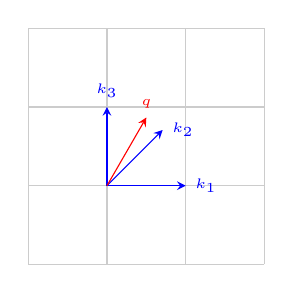
\begin{tikzpicture}

\draw[thin, gray!40] (-1, -1) grid (2, 2);
\draw[thin, blue, -stealth] (0, 0) -- (1, 0) node[anchor=west]{\tiny $k_1$};
\draw[thin, blue, -stealth] (0, 0) -- ({cos(90)}, {sin(90)}) node[anchor=south]{\tiny $k_3$};
\draw[thin, blue, -stealth] (0, 0) -- ({cos(45)}, {sin(45)}) node[anchor=west]{\tiny $k_2$};

\draw[thin, red, -stealth] (0, 0) -- ({cos(60)}, {sin(60)}) node[anchor=south]{\tiny $q$};



\end{tikzpicture}	
\end{document}
